% === FIGURES ===
% MRM: max 10 items (figures + tables combined)
% Budget: 9 figures + 1 table = 10 items (FULL)
% Supplementary: atlas, simulation recovery, Fisher.
%
% Per Stephan (2026-05): MRM does not allow caption titles or bold lead-in;
% caption begins with a single summary sentence. Coloring convention used
% throughout: blue = normal tissue, red = tumor, orange = NUTS,
% green = MAP, gray/black = CRLB / ground-truth / reference.
% Captions shortened 2026-06-02 (don't fit on page); detail moved to text.

% --- Fig 1: Cohort Diffusivity Spectra by Tissue and Zone ---
\begin{figure}[p]
\centering
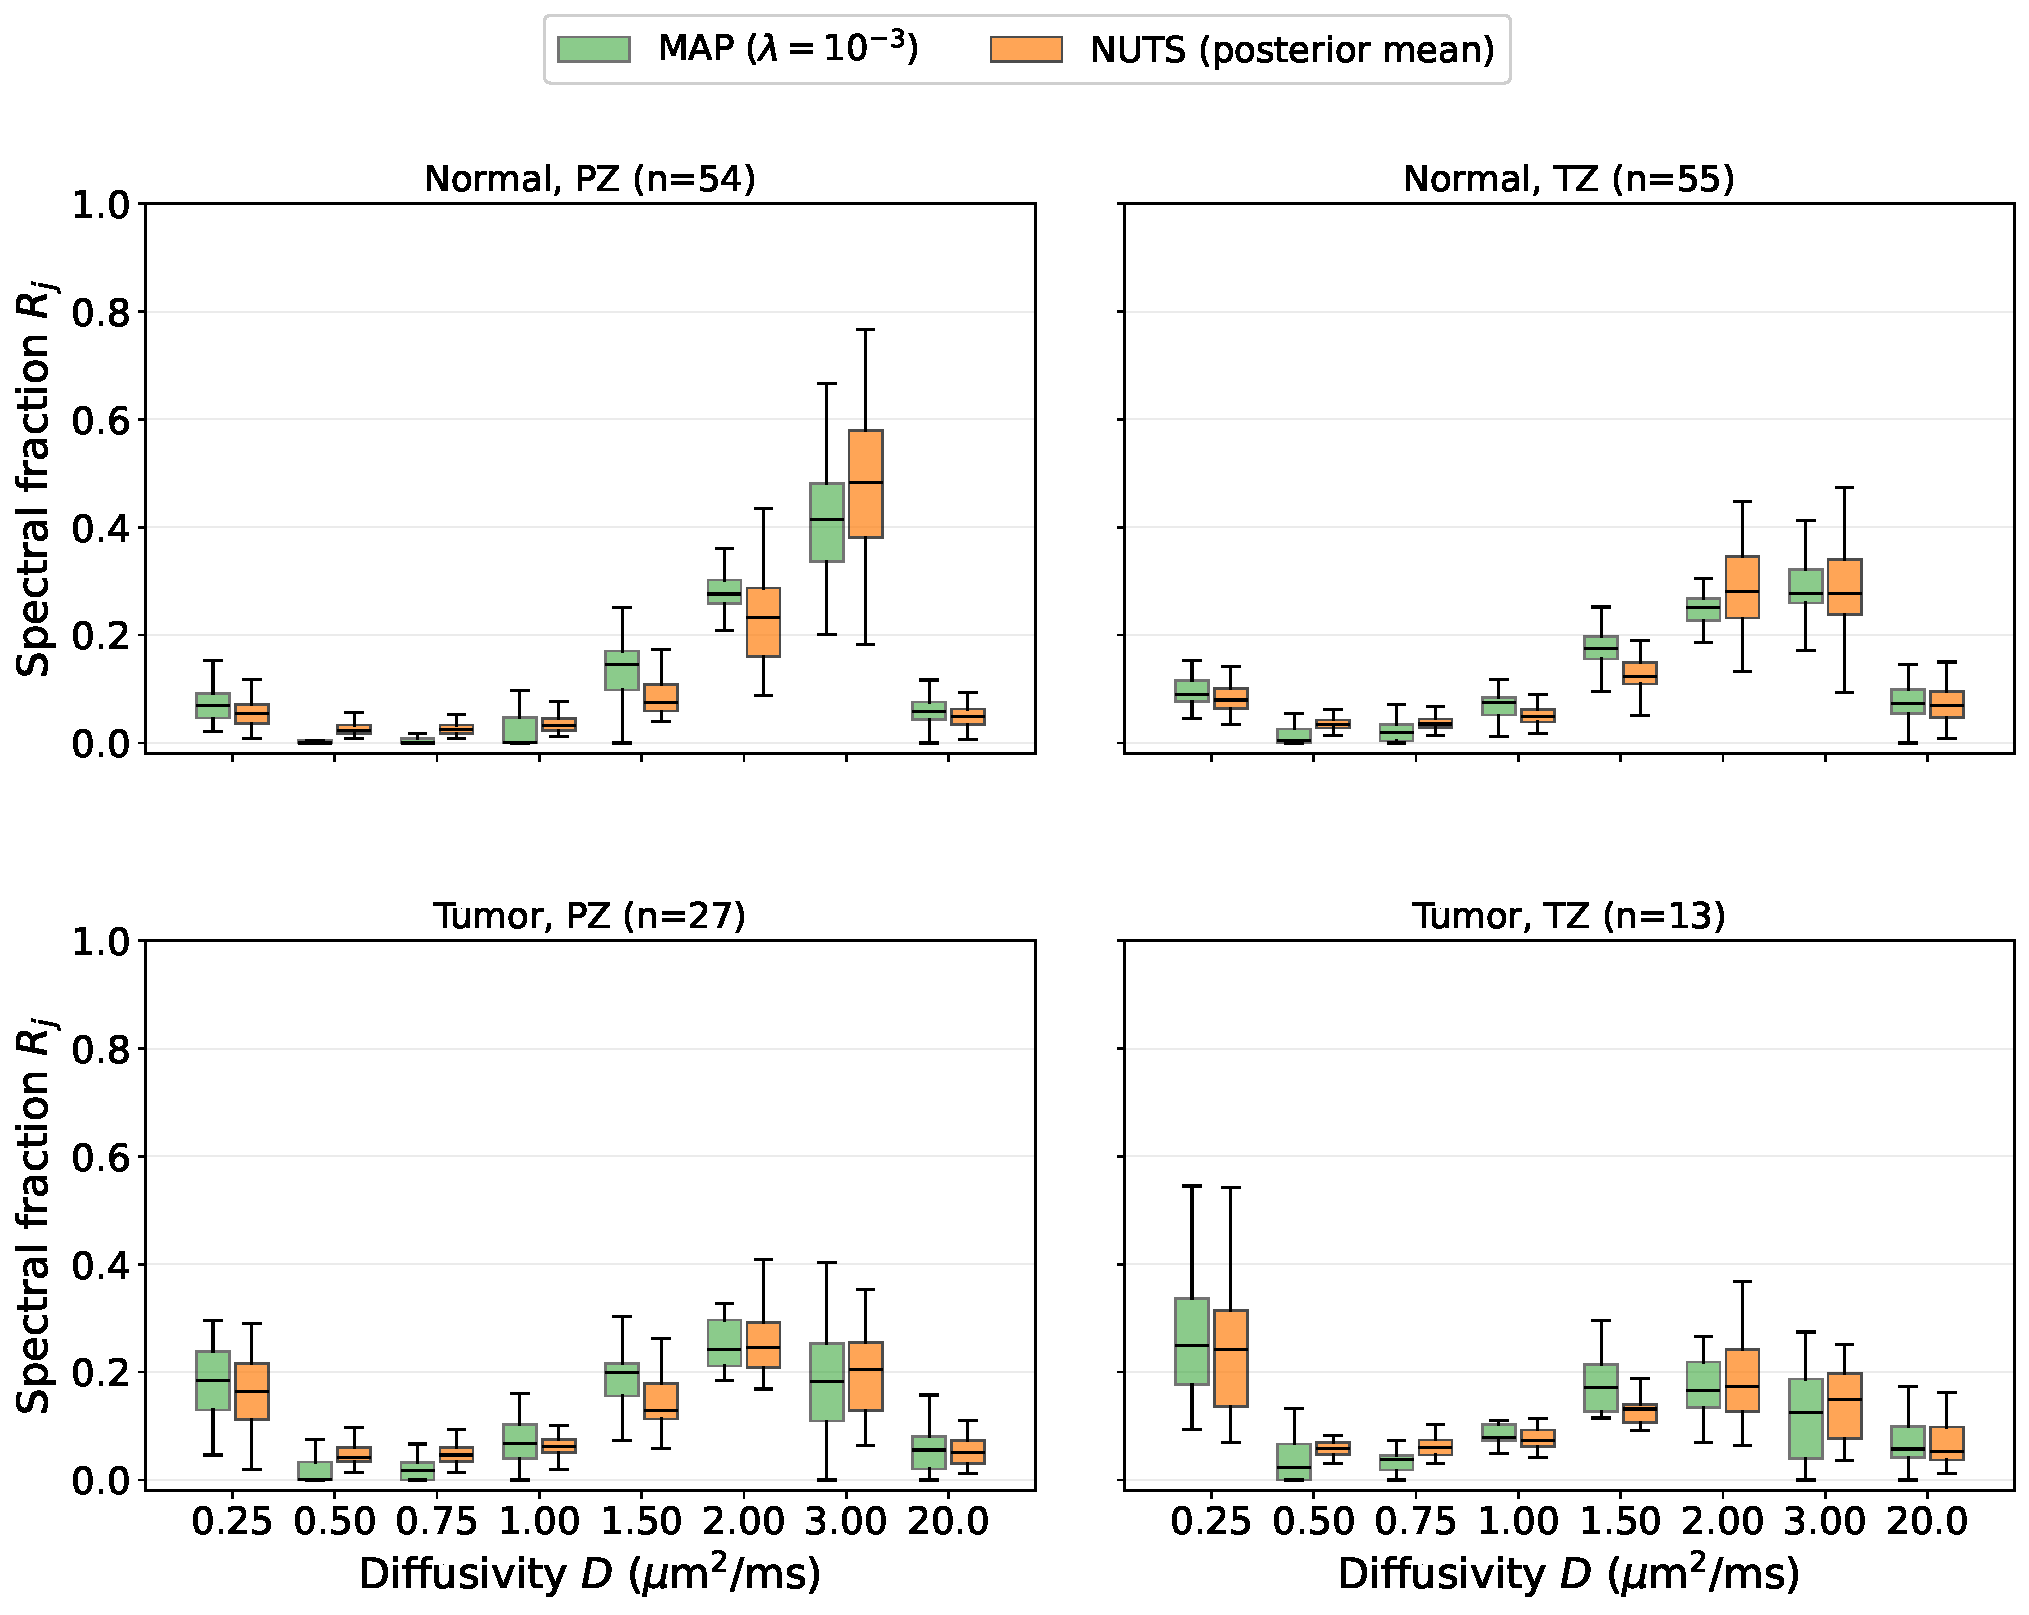
\includegraphics[width=\textwidth]{figures/fig1_v4.pdf}
\caption{%
Cohort diffusivity spectra by tissue type and anatomical zone.
For each diffusivity bin, box plots show the cohort distribution of the
estimated water fraction $R_j$ across ROIs (box: interquartile range; line:
median; whiskers: $1.5\times$ IQR), with MAP (green, hatched) alongside NUTS
posterior-mean estimates (orange) at the tuned regularization
$\lambda = 10^{-3}$.
Top row: normal; bottom row: tumor. Left column: peripheral zone (PZ); right:
transition zone (TZ).
Relative to normal tissue, tumor shows an elevated restricted-diffusion
fraction ($D = 0.25\;\umsmm$) and a reduced free-water fraction
($D = 3.0\;\umsmm$) in both zones, and MAP and NUTS agree closely.
Each box is the cohort distribution of the per-ROI posterior-mean fraction
(between-ROI spread); within-ROI posterior uncertainty is shown in
Figure~\ref{fig:sensitivity} and the supplementary atlas.
}
\label{fig:spectra}
\end{figure}

% --- Fig 2: Tumor-detection ROC; collapse onto the two outer compartments ---
\begin{figure}[p]
\centering
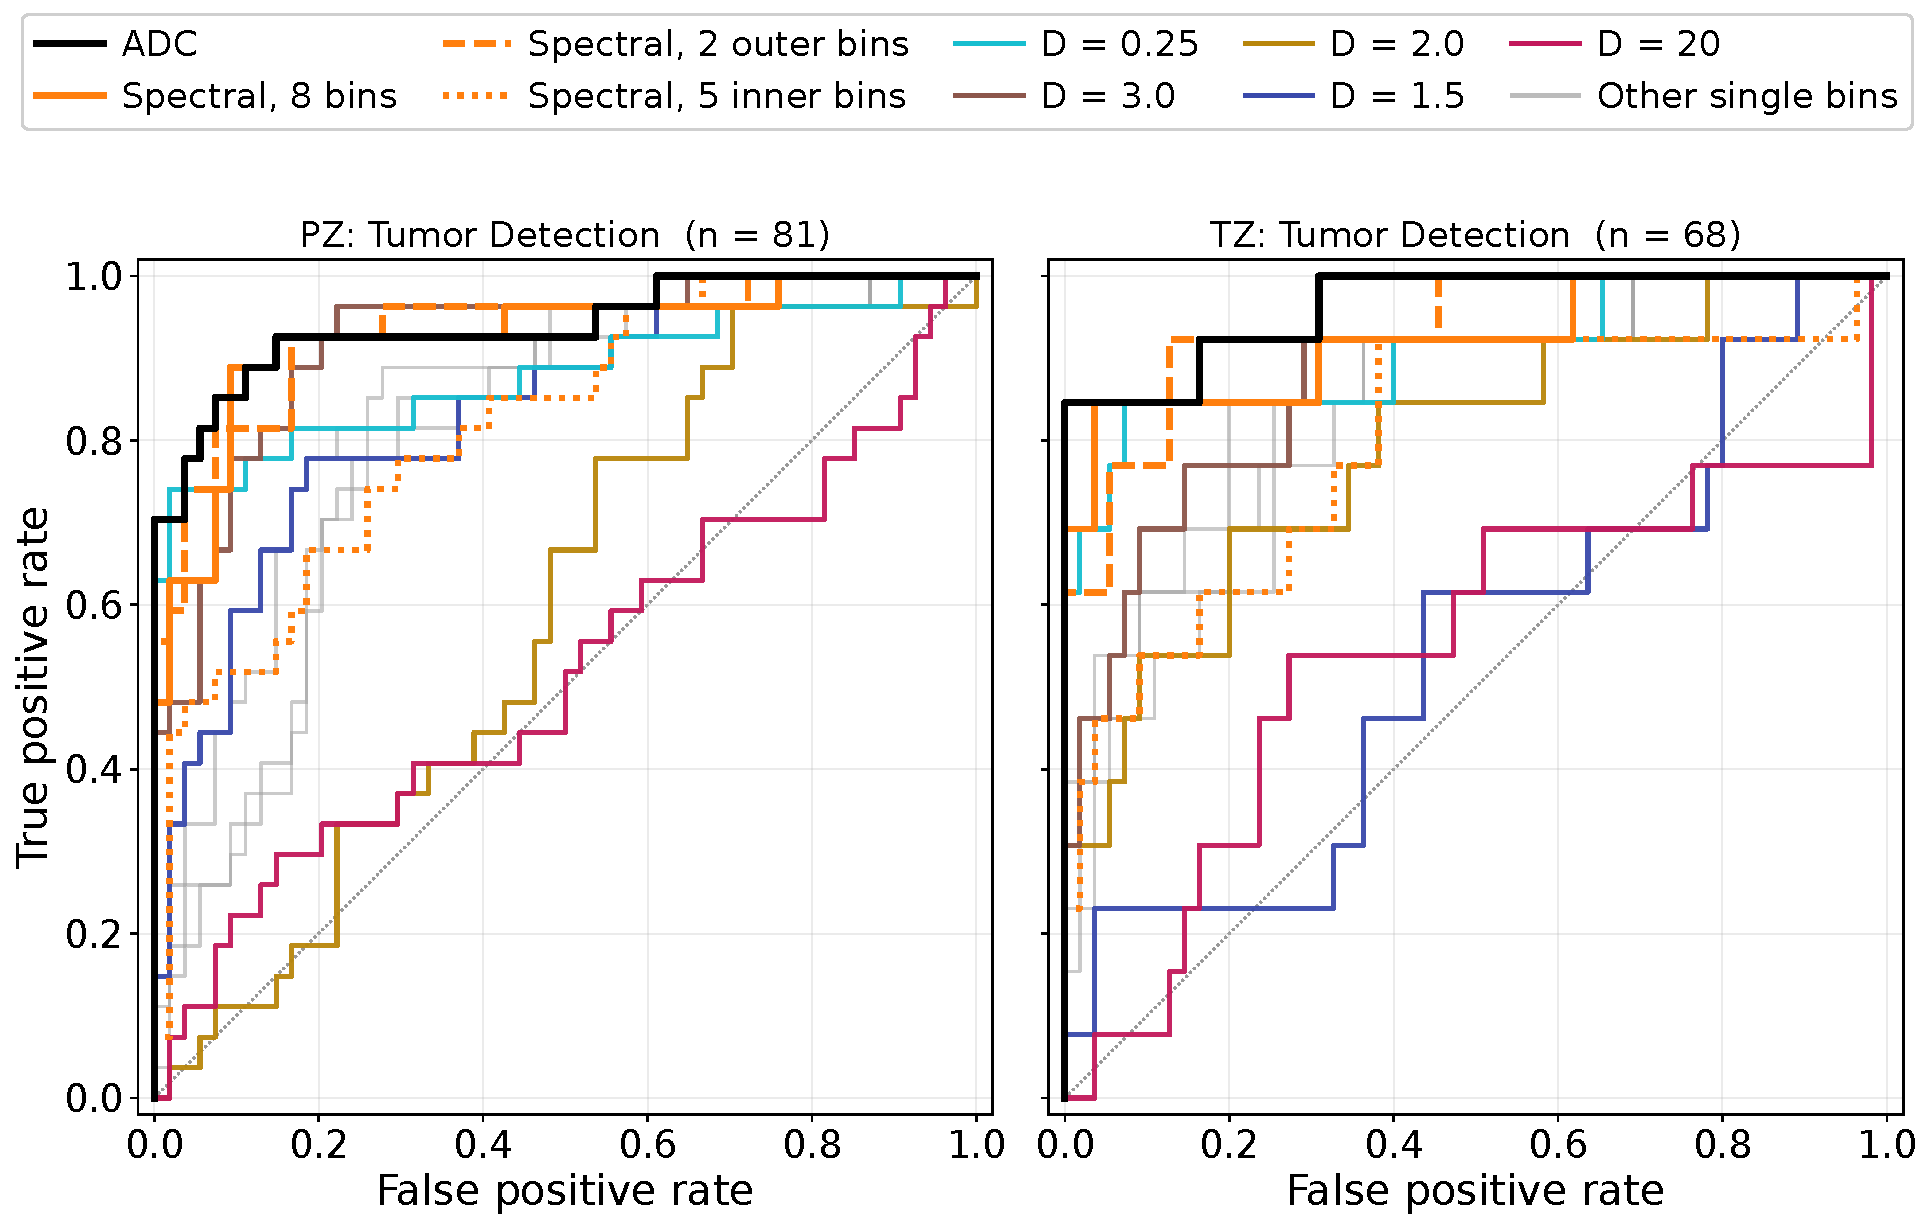
\includegraphics[width=\textwidth]{figures/fig2_v3.pdf}
\caption{%
Tumor detection collapses onto the two outer diffusivity compartments, and the
spectral classifier is equivalent to ADC.
Leave-one-out cross-validated ROC for tumor-versus-normal detection in the
peripheral zone (PZ, left; $n = 81$) and transition zone (TZ, right;
$n = 68$). The three thick reference curves---ADC (black), the spectral
classifier on all eight fractions (orange solid) and on only the two outer
fractions $\{D = 0.25,\,3.0\;\umsmm\}$ (orange dashed)---pass through the
identical NUTS-feature leave-one-out logistic-regression pipeline ($C = 1.0$)
for an apples-to-apples comparison.
The thin single-component curves are each a raw single-feature ROC in the
tumor-positive orientation (not the LOOCV pipeline): the strong outer
components $D = 0.25\;\umsmm$ (restricted, teal) and $D = 3.0\;\umsmm$
(free water, brown), the two weakest bins $D = 2.0\;\umsmm$ (goldenrod) and
$D = 20\;\umsmm$ (magenta), which sit near chance and carry essentially no
detection signal, and the remaining intermediate bins as a faint grey bundle.
The three thick curves are statistically indistinguishable and the
two-fraction classifier matches the full eight-fraction one: the intermediate
and free-water fractions add nothing to detection.
AUC values with 95\% confidence intervals are reported in
Table~\ref{tab:auc}.
}
\label{fig:roc}
\end{figure}

% --- Fig 3: ADC vs Spectral Discriminant ---
\begin{figure}[p]
\centering
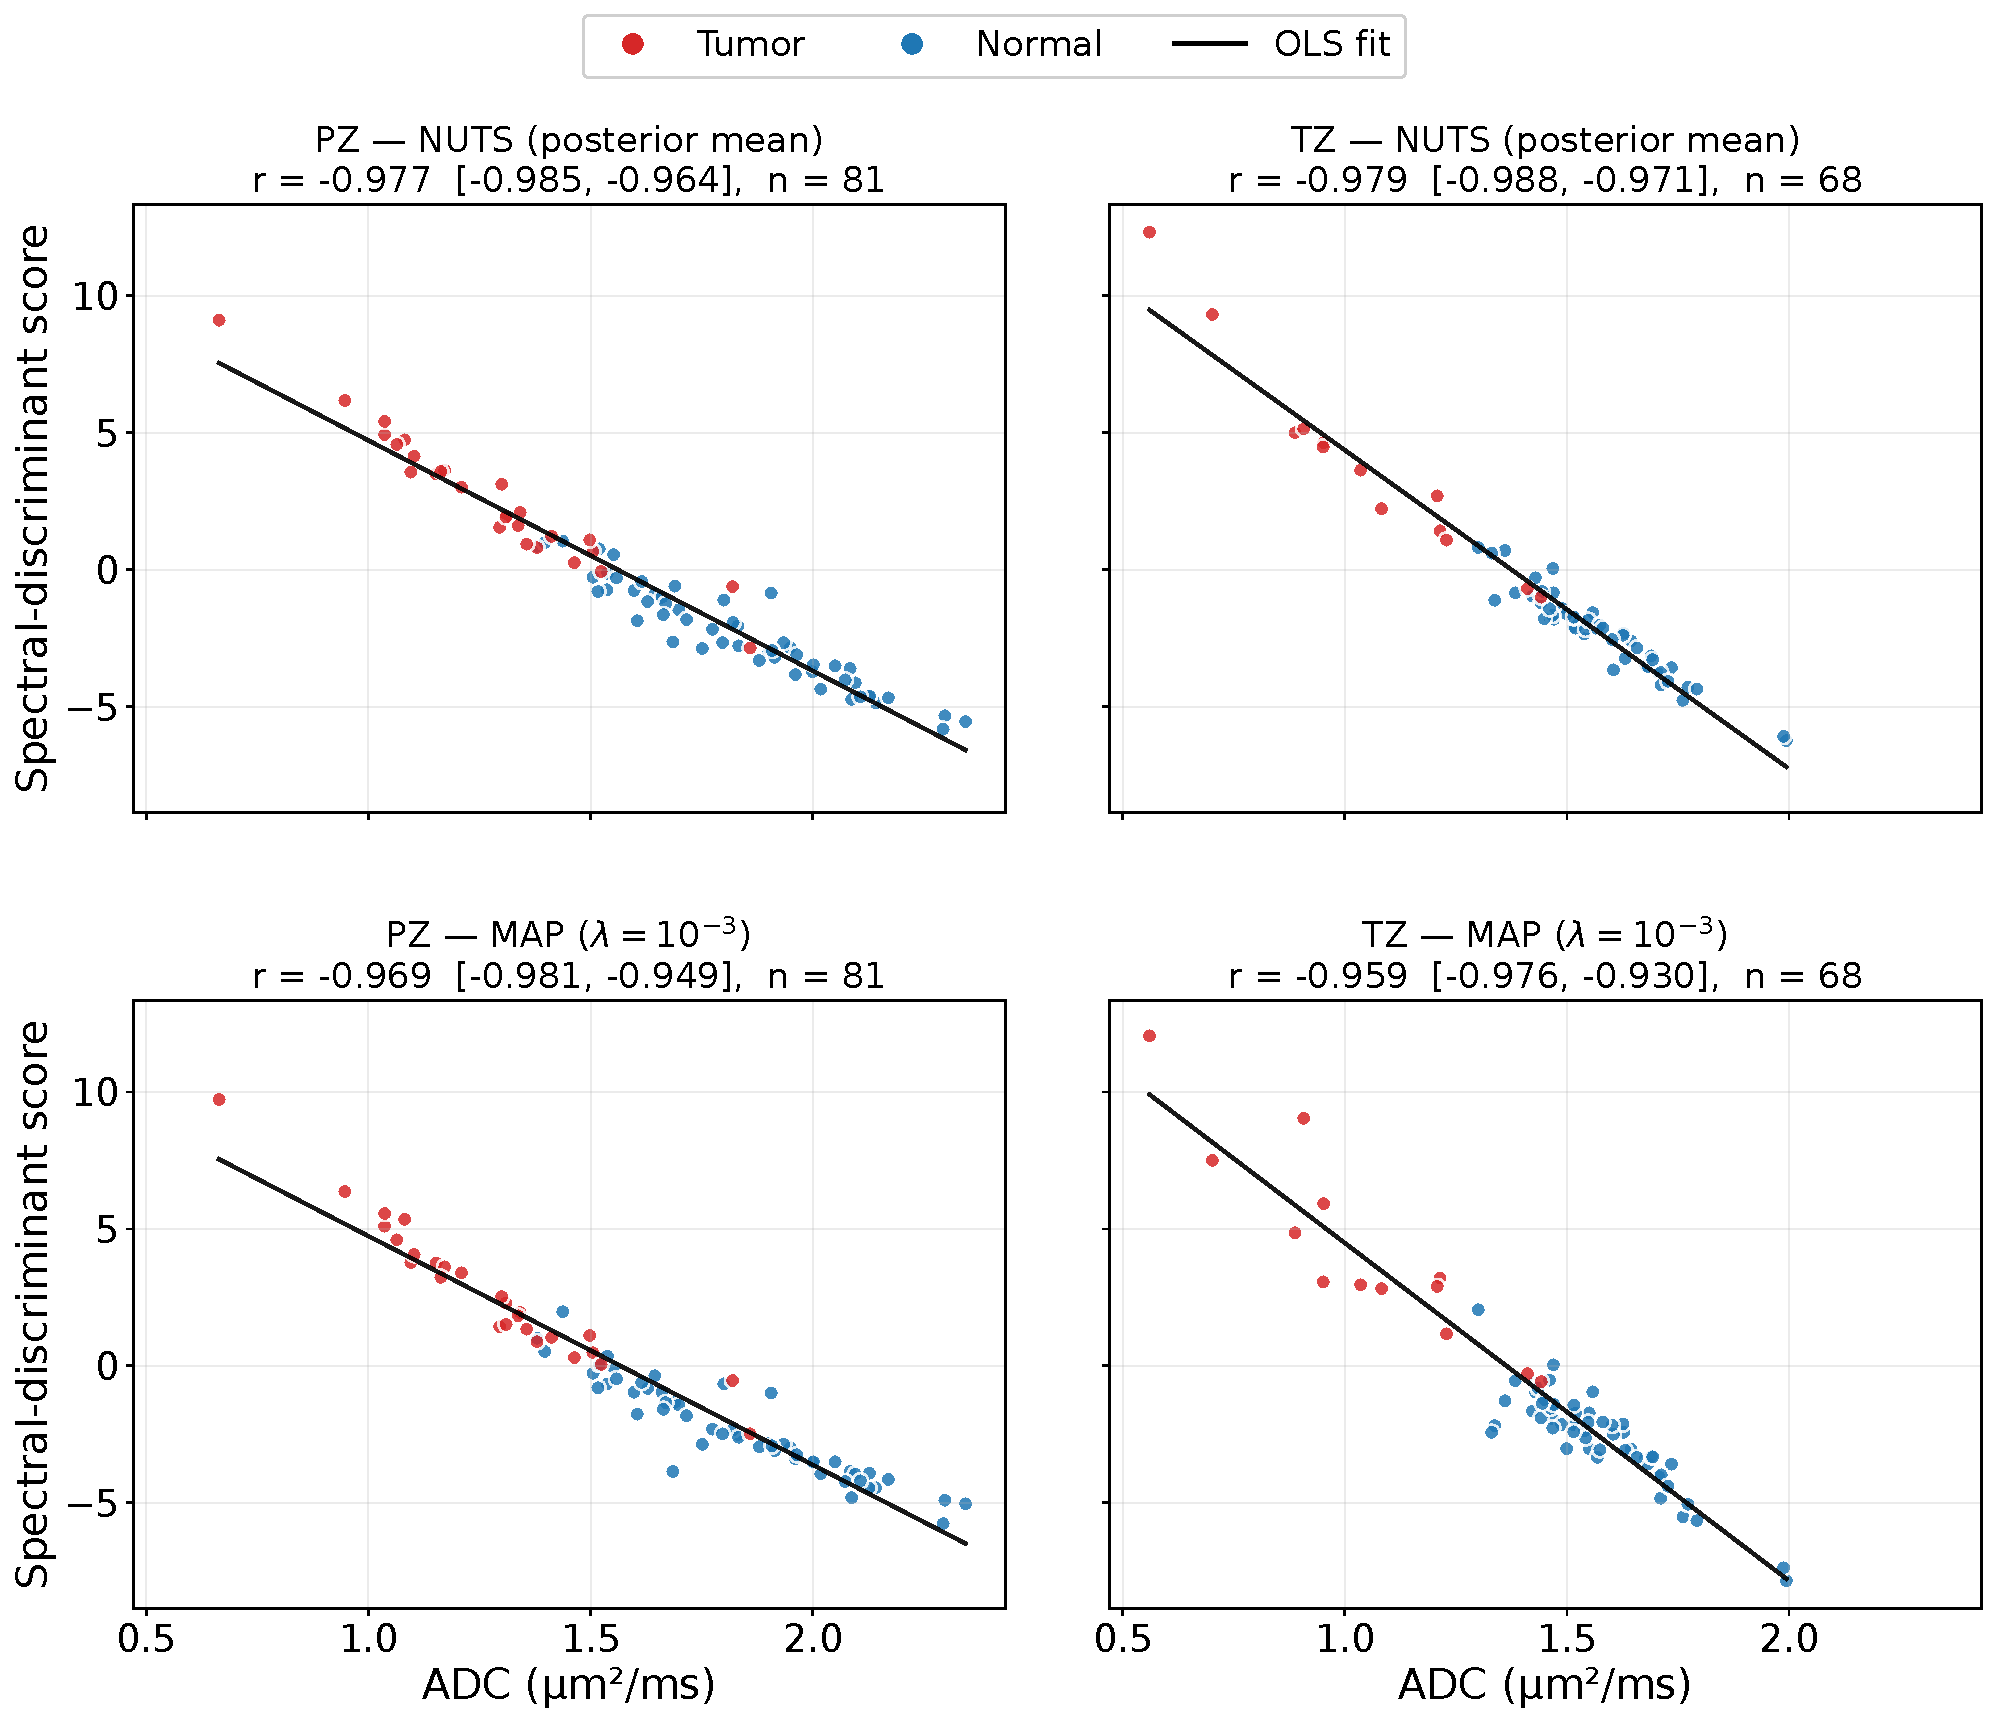
\includegraphics[width=\textwidth]{figures/fig3_v4.pdf}
\caption{%
ADC is a near-optimal spectral discriminant, and the equivalence holds for
both estimators.
ADC versus the spectral discriminant score (logistic-regression linear
predictor from the eight spectral fractions) across ROIs, by anatomical zone
(columns: PZ, $n = 81$, left; TZ, $n = 68$, right) and spectral estimator
(rows: NUTS posterior-mean, top; constrained-MAP at tuned
$\lambda = 10^{-3}$, bottom).
All panels share common axes; the discriminant is fit separately per zone and
estimator, so its score scale is comparable only within a panel, whereas ADC
($x$-axis) is the same physical quantity throughout.
Tumor ROIs (red) cluster at low ADC and high discriminant, normal ROIs (blue)
the reverse; the black line is the OLS fit.
Per-panel Pearson $r$ with a 95\% percentile-bootstrap confidence interval is
annotated in each panel (all $|r| > 0.95$).
The near-perfect anti-correlation shows that ADC rank-orders ROIs almost
identically to the spectral classifier, independent of estimator.
}
\label{fig:adc_discriminant}
\end{figure}

% --- Fig 4: per-bin anatomy of the spectral discriminant ---
\begin{figure}[p]
\centering
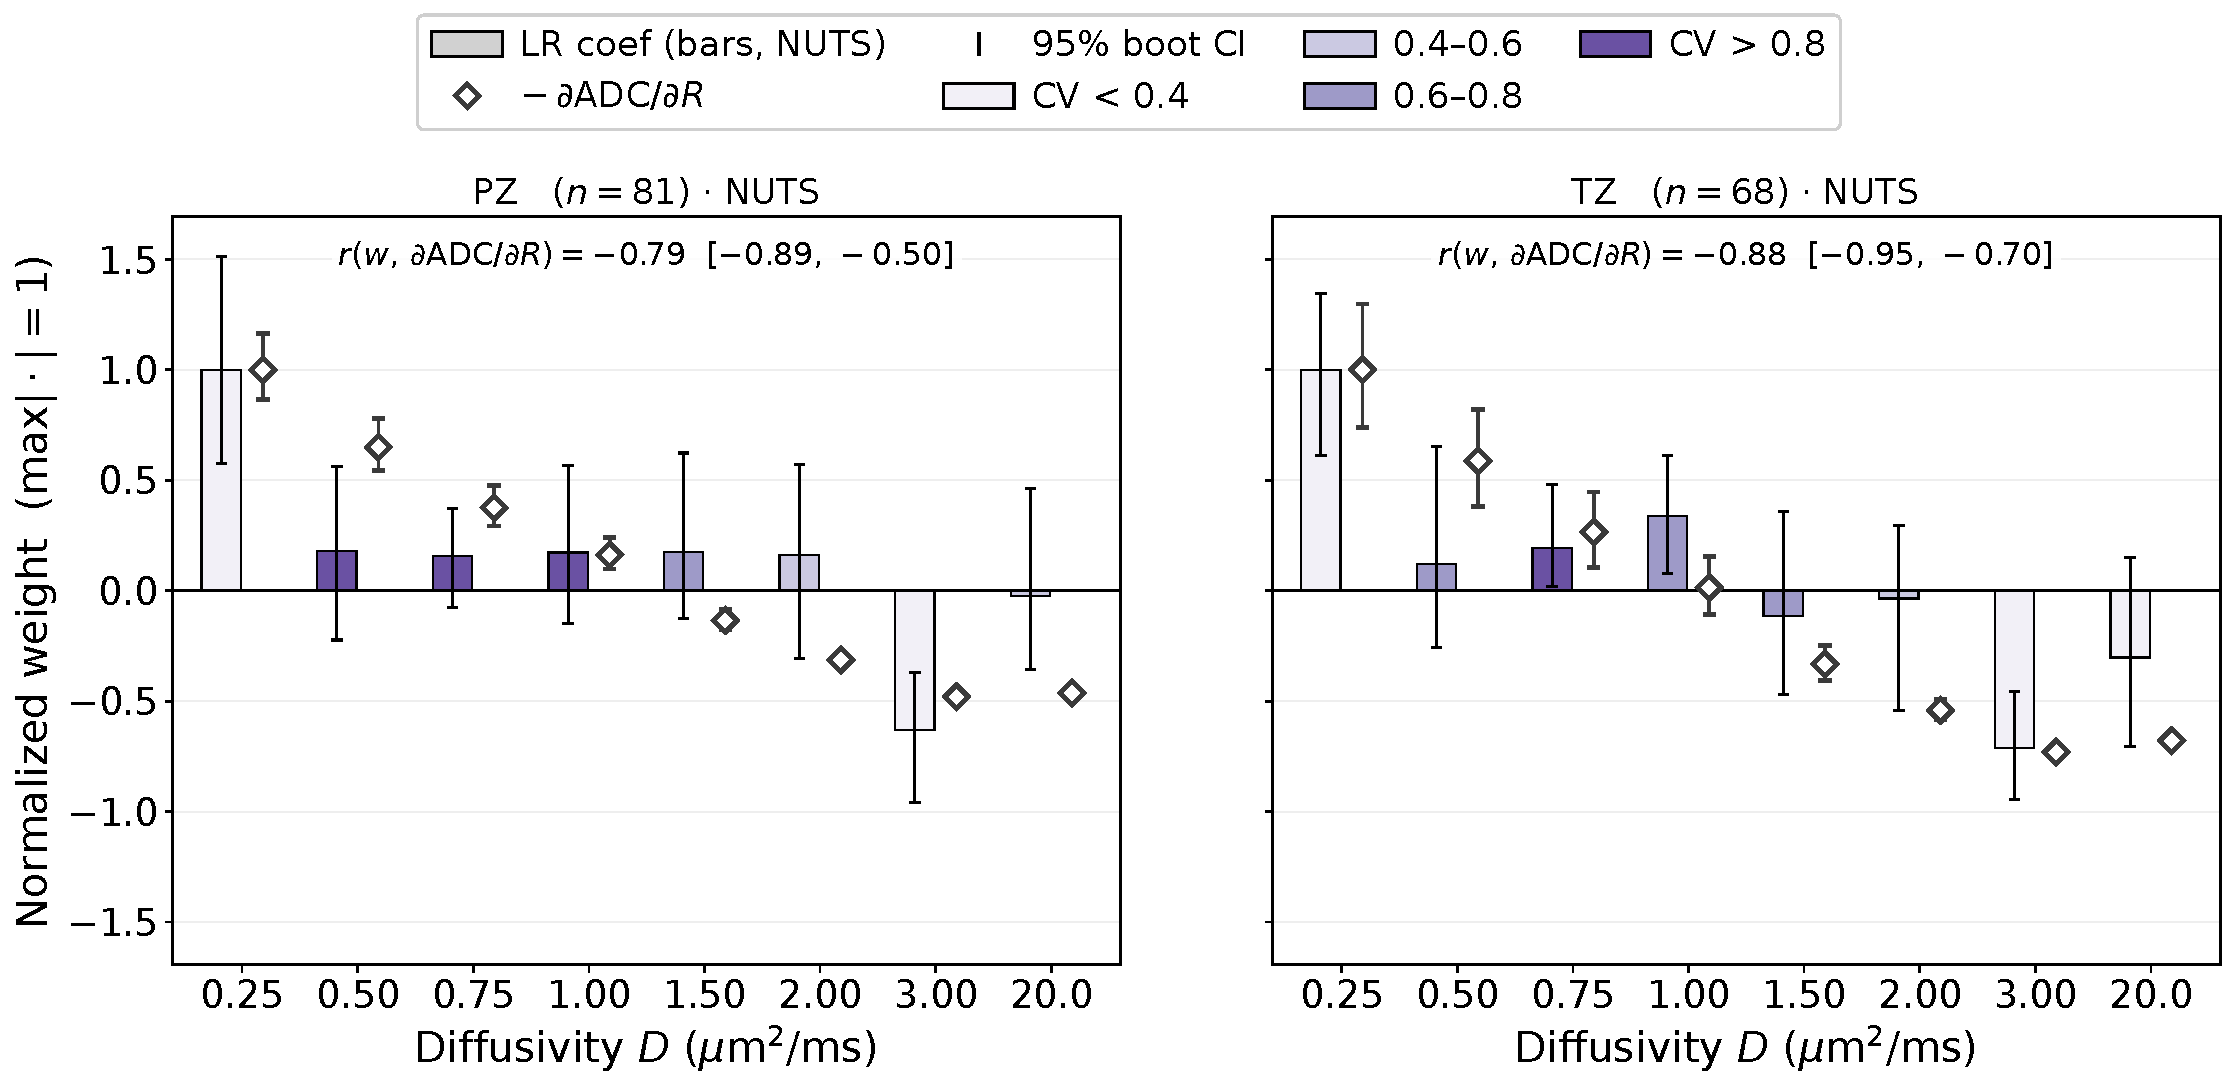
\includegraphics[width=\textwidth]{figures/fig4_std_v4.pdf}
\caption{%
The spectral discriminant is statistically a two-compartment detector, and its
two stable bins coincide with where ADC is most sensitive.
For each zone (PZ, TZ), bars give the standardized tumor-versus-normal
logistic-regression coefficient per diffusivity bin (NUTS features, $C = 1.0$,
the same fit as Figure~\ref{fig:adc_discriminant}), normalized to
$\max|w| = 1$, with 95\% bootstrap confidence intervals.
Charcoal diamonds give the ADC sensitivity $-\partial\text{ADC}/\partial R_j$
at the average tumor spectrum (normalized, sign-aligned to the tumor
direction).
Each bar is colored and hatched by the bin's within-ROI posterior CV (light
$=$ well identified to dark $=$ poorly identified), a per-ROI identifiability
distinct from the cohort-level coefficient stability shown by the bootstrap
intervals.
In both zones only the two outer bins carry stable weight ($D = 0.25\;\umsmm$
positive, $D = 3.0\;\umsmm$ negative); the intermediate coefficients are
individually unstable from inter-bin collinearity and poor identifiability, so
their separate detection weights are not attributable.
The profile anti-correlates with $\partial\text{ADC}/\partial R_j$
($r = -0.79$ PZ, $-0.88$ TZ), carried by the two outer bins---weaker than the
near-unity value seen under heavy regularization ($\lambda = 0.1$), where
smearing artificially smooths the profile (see Discussion).
The intermediate bins' value appears instead as a grading signal
(Figure~\ref{fig:spectrum_ggg}).
}
\label{fig:sensitivity}
\end{figure}

% --- Fig 5: Diffusivity Spectrum by Gleason Grade Group (single-panel ladder) ---
\begin{figure}[p]
\centering
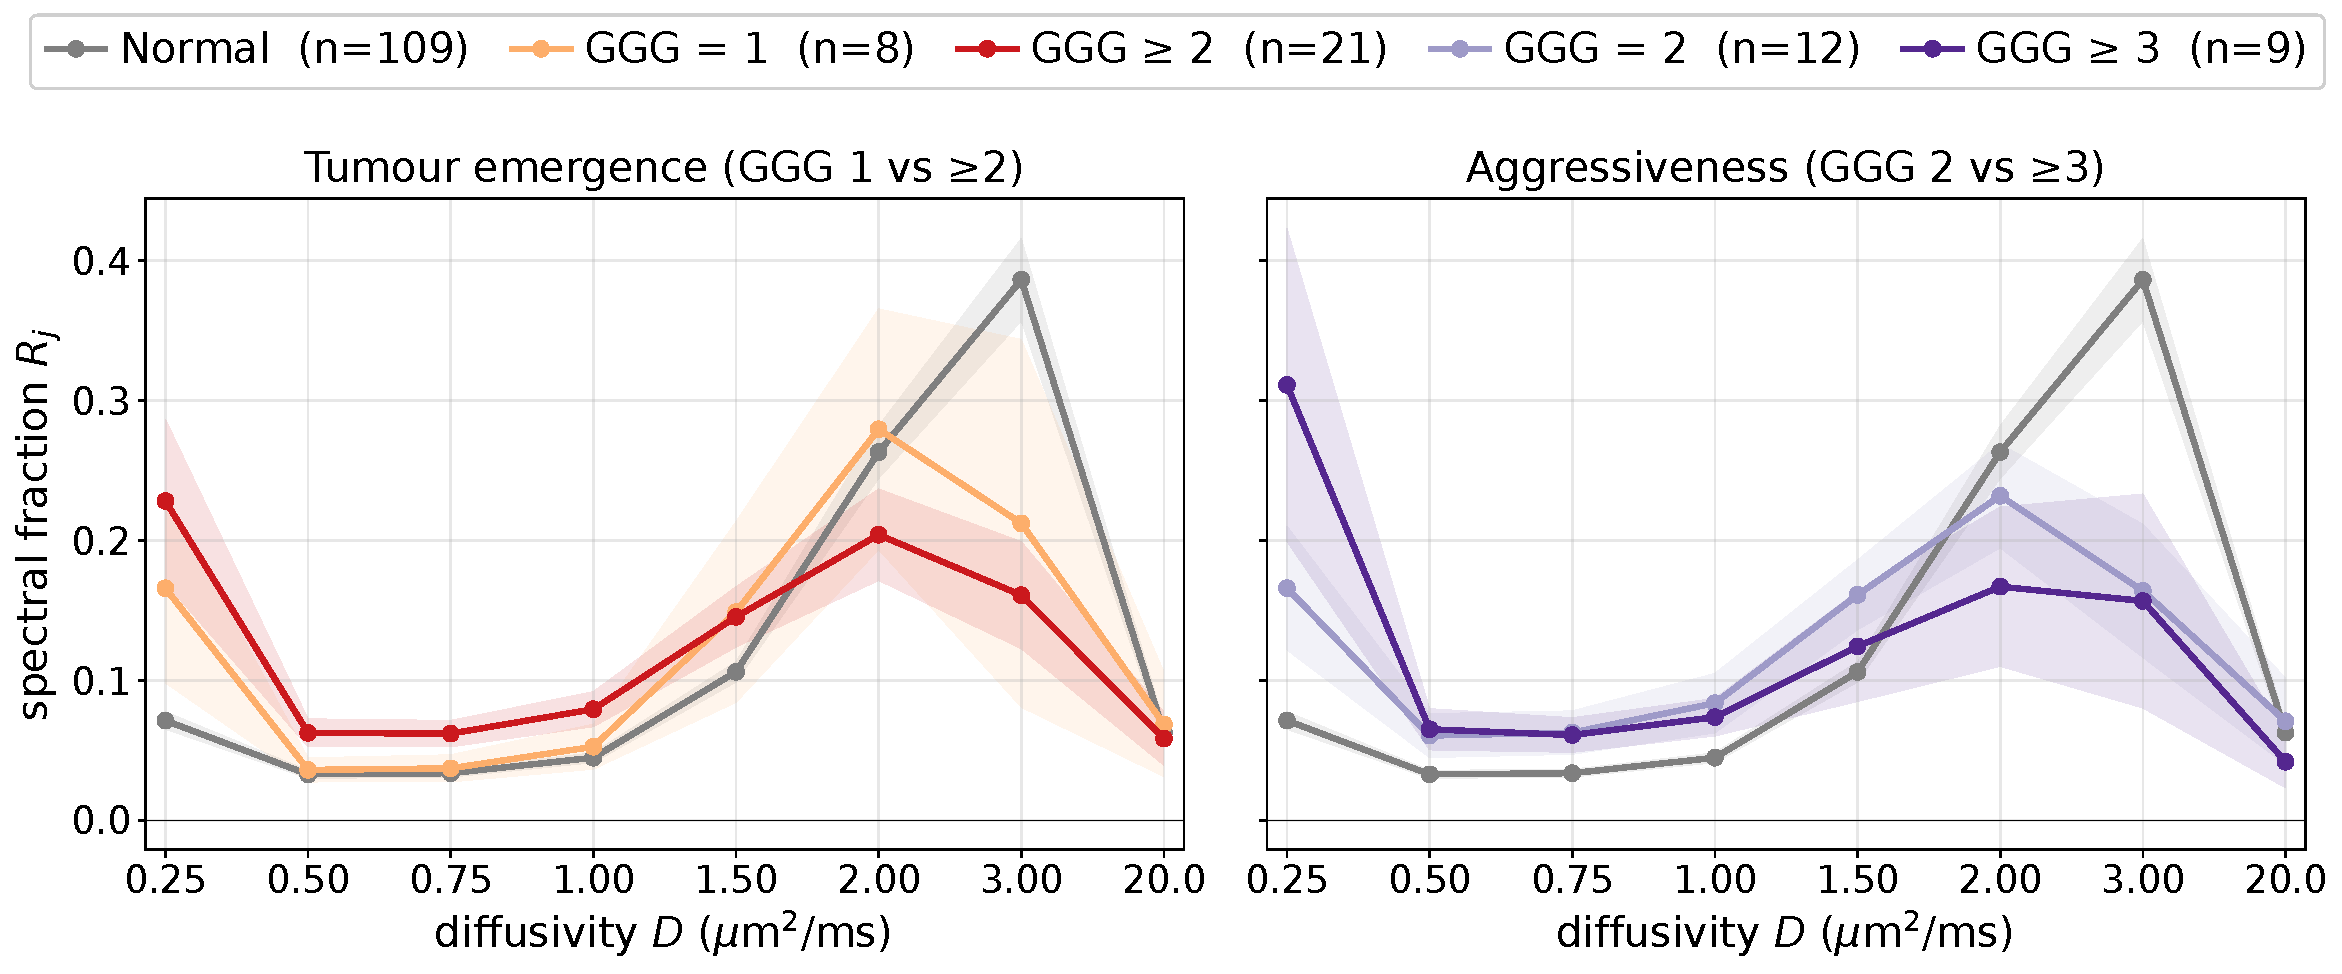
\includegraphics[width=\textwidth]{figures/fig5_v5.pdf}
\caption{%
The diffusivity spectrum by Gleason Grade Group reveals a detection axis
distinct from a grading axis.
NUTS posterior-mean spectrum averaged across ROIs, in two contrasts that share
a normal-tissue baseline (gray, $n = 109$). Left (emergence): GGG\,$=\,1$
($n = 8$) versus GGG\,$\geq 2$ ($n = 21$). Right (aggressiveness): GGG\,$=\,2$
($n = 12$) versus GGG\,$\geq 3$ ($n = 9$). Each grade group has its own color.
Shaded bands are 95\% confidence intervals of the group mean (Student's $t$,
$\text{df} = n - 1$).
The free-water bin ($D = 3.0\;\umsmm$, a proxy for intact gland lumen)
collapses at tumor onset ($0.39$ normal $\to 0.21$ at GGG\,$=\,1$) and changes
little thereafter ($0.16$ at GGG\,$\geq 3$): it carries detection, not grade.
In contrast the restricted-cellular bin ($D = 0.25\;\umsmm$) and the
glandular-epithelial bin ($D = 2.0\;\umsmm$), where ADC is least sensitive,
track grade: $D = 0.25$ rises with grade ($0.07$ normal, $0.17$ at
GGG\,$=\,1$--$2$, $0.31$ at GGG\,$\geq 3$) and $D = 2.0$ is preserved in
low-grade tumor then depleted ($0.26$ normal, $0.28$ at GGG\,$=\,1$, $0.17$ at
GGG\,$\geq 3$).
Grade groups are small (down to $n = 8$--$9$) and the bands wide; 11 of 40
tumor ROIs (7 with GGG\,$=\,0$, 4 ungraded) are not shown.
}
\label{fig:spectrum_ggg}
\end{figure}

% --- Fig 6: Uncertainty-aware classifier (posterior propagation) ---
\begin{figure}[p]
\centering
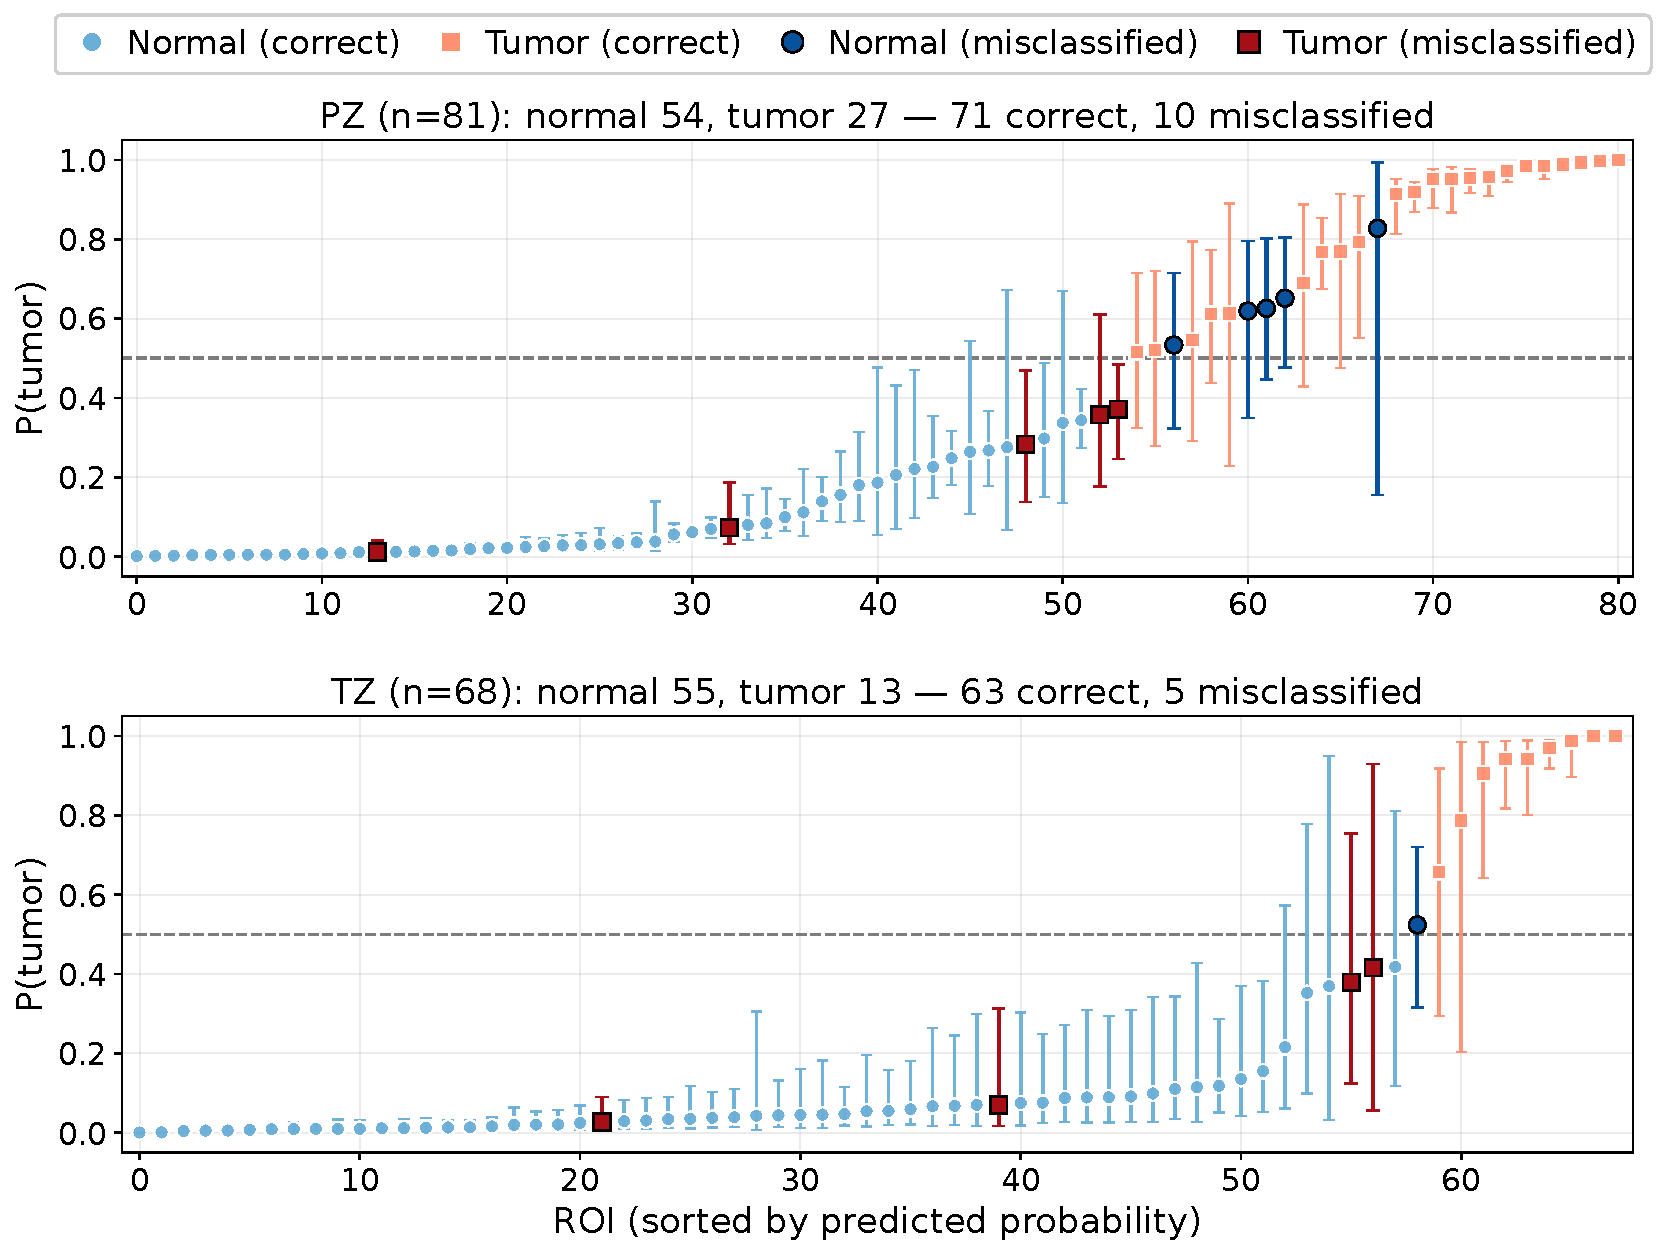
\includegraphics[width=\textwidth]{figures/fig6_v2.pdf}
\caption{%
Propagating the diffusivity-spectrum posterior through the classifier turns a
binary label into a calibrated probability of cancer whose uncertainty is
largest where the classifier is most likely to be wrong.
For each ROI the leave-one-out classifier (the same NUTS-feature pipeline as
Figure~\ref{fig:roc}, $C = 1$) is applied to every NUTS posterior draw of the
eight fractions, yielding a posterior distribution over $P(\mathrm{tumor})$
rather than a point estimate.
Per-ROI predictions in the peripheral zone (top, $n = 81$) and transition zone
(bottom, $n = 68$), each ROI sorted by its predicted probability: markers at
the posterior-mean probability (circles normal, squares tumor) with error bars
the propagated 90\% credible interval; correctly classified ROIs are shown in
pale colors and misclassified ROIs in saturated colors.
Two uncertainties are evident. First, the credible interval is on average
$2.4\times$ wider for misclassified than for correctly classified ROIs (pooled
mean width $0.39$ vs $0.16$; Welch $p = 0.003$). Second, intervals widen toward
the decision boundary ($P = 0.5$); this widening is partly a geometric property
of the logistic link---in logit space both the boundary effect and the
misclassified-to-correct width ratio shrink markedly---but a genuine residual
remains.
The residual confidently-misclassified ROIs are almost all low-grade or
ungraded tumors whose spectra resemble normal tissue
(cf.\ Figure~\ref{fig:spectrum_ggg})---a limit of diffusion contrast, not a
failure of the uncertainty estimate.
A MAP point estimate cannot produce these intervals.
This analysis is exploratory.
}
\label{fig:uncertainty}
\end{figure}

% --- Fig 7: Direction independence (whole-ROI) ---
% Generator: scripts/fig7_directions_roi.py (decodes the per-direction ROI .dat
% export; MAP spectra via recompute.compute_map_spectrum). Patient 9283, the
% only matched same-zone (PZ) normal+tumour pair. Aggregate per-direction CV
% over all 13 ROIs is reported in Results.
\begin{figure}[p]
\centering
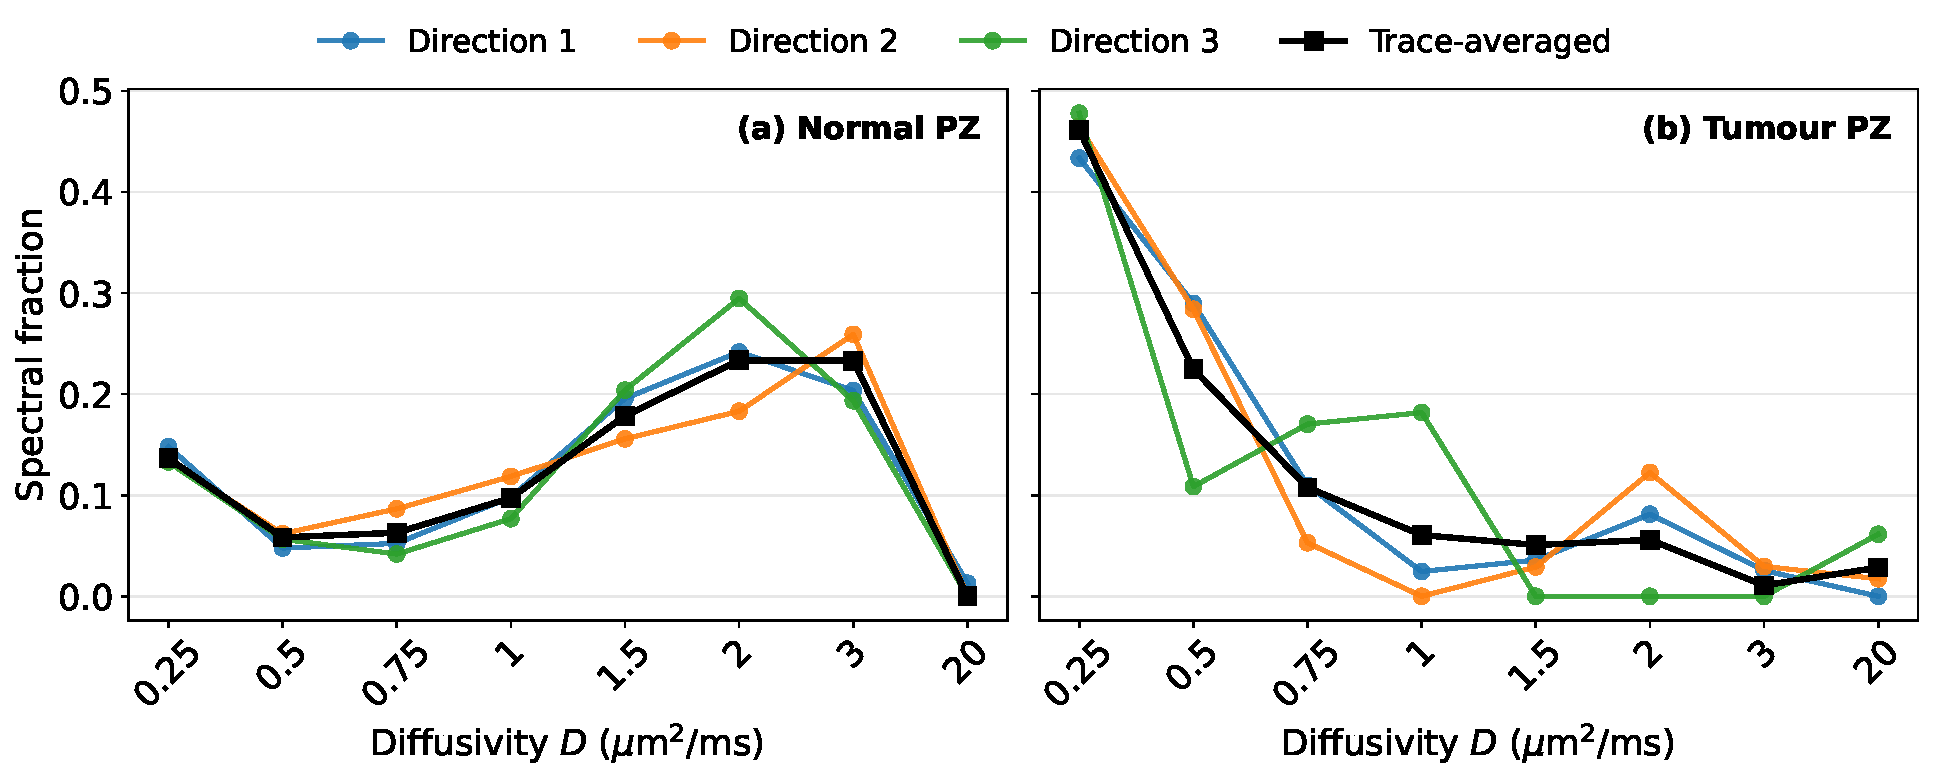
\includegraphics[width=\textwidth]{figures/fig_directions_v2.pdf}
\caption{%
Direction independence of whole-ROI spectral estimates validates trace
averaging.
Per-encoding-direction MAP spectra (three encoding directions) versus the
trace-averaged spectrum (black) for (a)~a normal and (b)~a tumor
peripheral-zone region of interest in a representative patient.
The three directions agree closely in the diagnostically dominant
restricted-diffusion bin ($D = 0.25\;\umsmm$; mean direction-wise CV $9\%$
across all 13 regions); the larger inter-direction spread in the intermediate
and near-empty bins ($D = 0.5$--$2.0$ and $D = 20\;\umsmm$) mirrors their poor
identifiability rather than reflecting genuine anisotropy, the per-direction
CV tracking each bin's inverse mass.
Because tumor detection rests on the well-identified outer compartments, trace
averaging is well justified; aggregate per-bin statistics are reported in
Results.
MAP estimates are shown (constrained ridge, $\lambda = 10^{-3}$); MAP and NUTS
are equivalent on realistic spectra (Figure~\ref{fig:validation}).
}
\label{fig:directions}
\end{figure}

% --- Fig 8: Method validation on simulated ground truth (spectrum x SNR battery) ---
% Generator: scripts/fig8_battery.py (replots from cached
% results/simulation/fig8_battery_snr.npz; --regen resamples). 4 ground truths
% x 2 SNR recovery grid + joint-noise sigma-calibration panel. No Gibbs
% (deferred). Real pipeline: nuts.yaml + tuned-MAP ridge.yaml.
\begin{figure}[p]
\centering
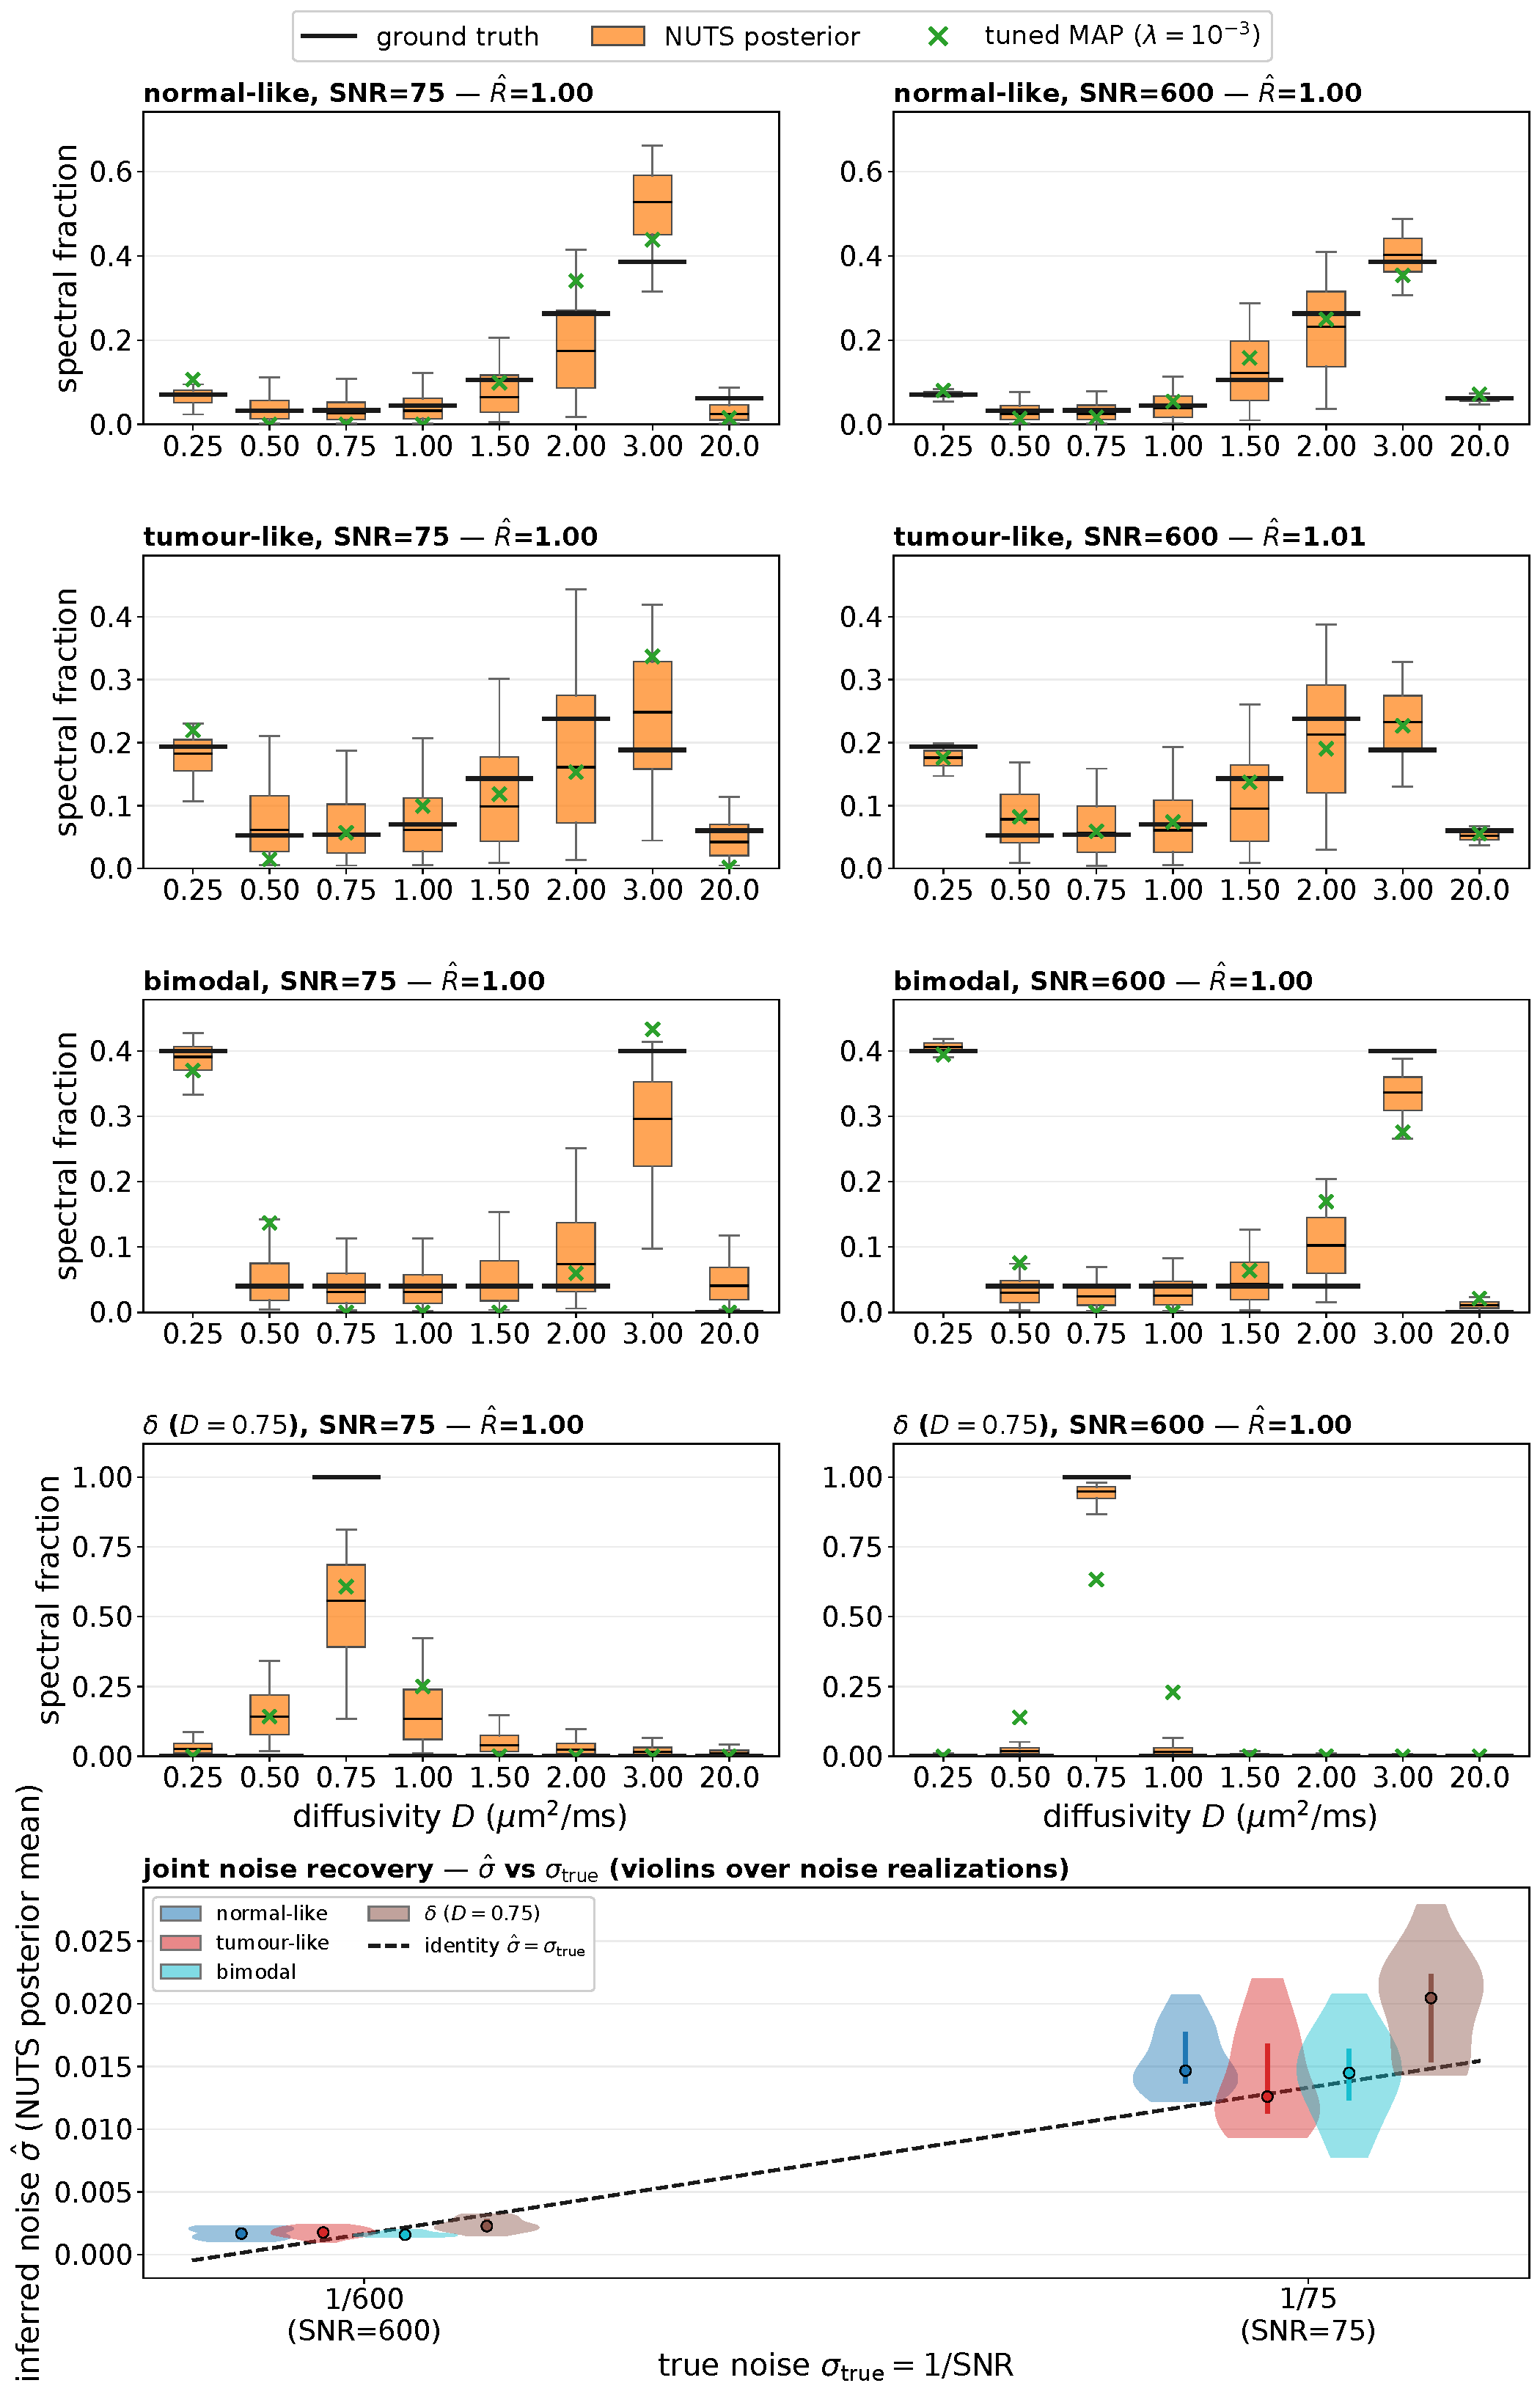
\includegraphics[width=\textwidth]{figures/fig8_v5.pdf}
\caption{%
Validation of the Bayesian spectral inference on simulated ground truth across
spectrum shape and signal-to-noise ratio.
Four ground-truth spectra---a normal-like and a tumor-like spectrum (the
cohort-mean NUTS spectra), a bimodal spectrum (mass at $D = 0.25$ and
$3.0\;\umsmm$), and a concentrated $\delta$ at $D = 0.75\;\umsmm$---are each
recovered at a low (SNR $= 75$) and a high (SNR $= 600$) noise level that
bracket the cohort median (303).
In each panel the black marks are the truth, the orange box plots the NUTS
posterior for one noisy realization (box $=$ interquartile range, whiskers
$=$ 5th--95th percentile), and the green cross the tuned-MAP estimate
($\lambda = 10^{-3}$); the split-$\hat{R}$ convergence diagnostic is reported
in each panel title (all $\hat{R} \leq 1.01$).
The smooth spectra are recovered well at both SNRs (tighter at high SNR),
whereas the $\delta$ spike is under-recovered and smeared into its correlated
neighboring bins---the genuine identifiability limit of this b-value grid, not
a sampler artifact.
The bottom panel shows joint noise inference: the inferred noise
$\hat{\sigma}$ (NUTS posterior mean over 12 realizations per condition, drawn
as violins) versus the true $\sigma = 1/\mathrm{SNR}$ (dashed identity line).
$\sigma$ is recovered to within $\sim$10\% for the smooth spectra but is
over-estimated by $\sim$35--50\% on the $\delta$, where the model absorbs the
unrepresentable spike as excess noise (consistent with the coverage caveat
discussed below).
}
\label{fig:validation}
\end{figure}

% --- Fisher Information Analysis: lives in the Supplement (sections/supporting.tex) ---
% The \label{fig:fisher} is defined there, so the in-text references in
% theory/results/discussion resolve to a supplementary figure.

% --- Fig 9: Pixel-wise Spectral Decomposition ---
\begin{figure}[p]
\centering
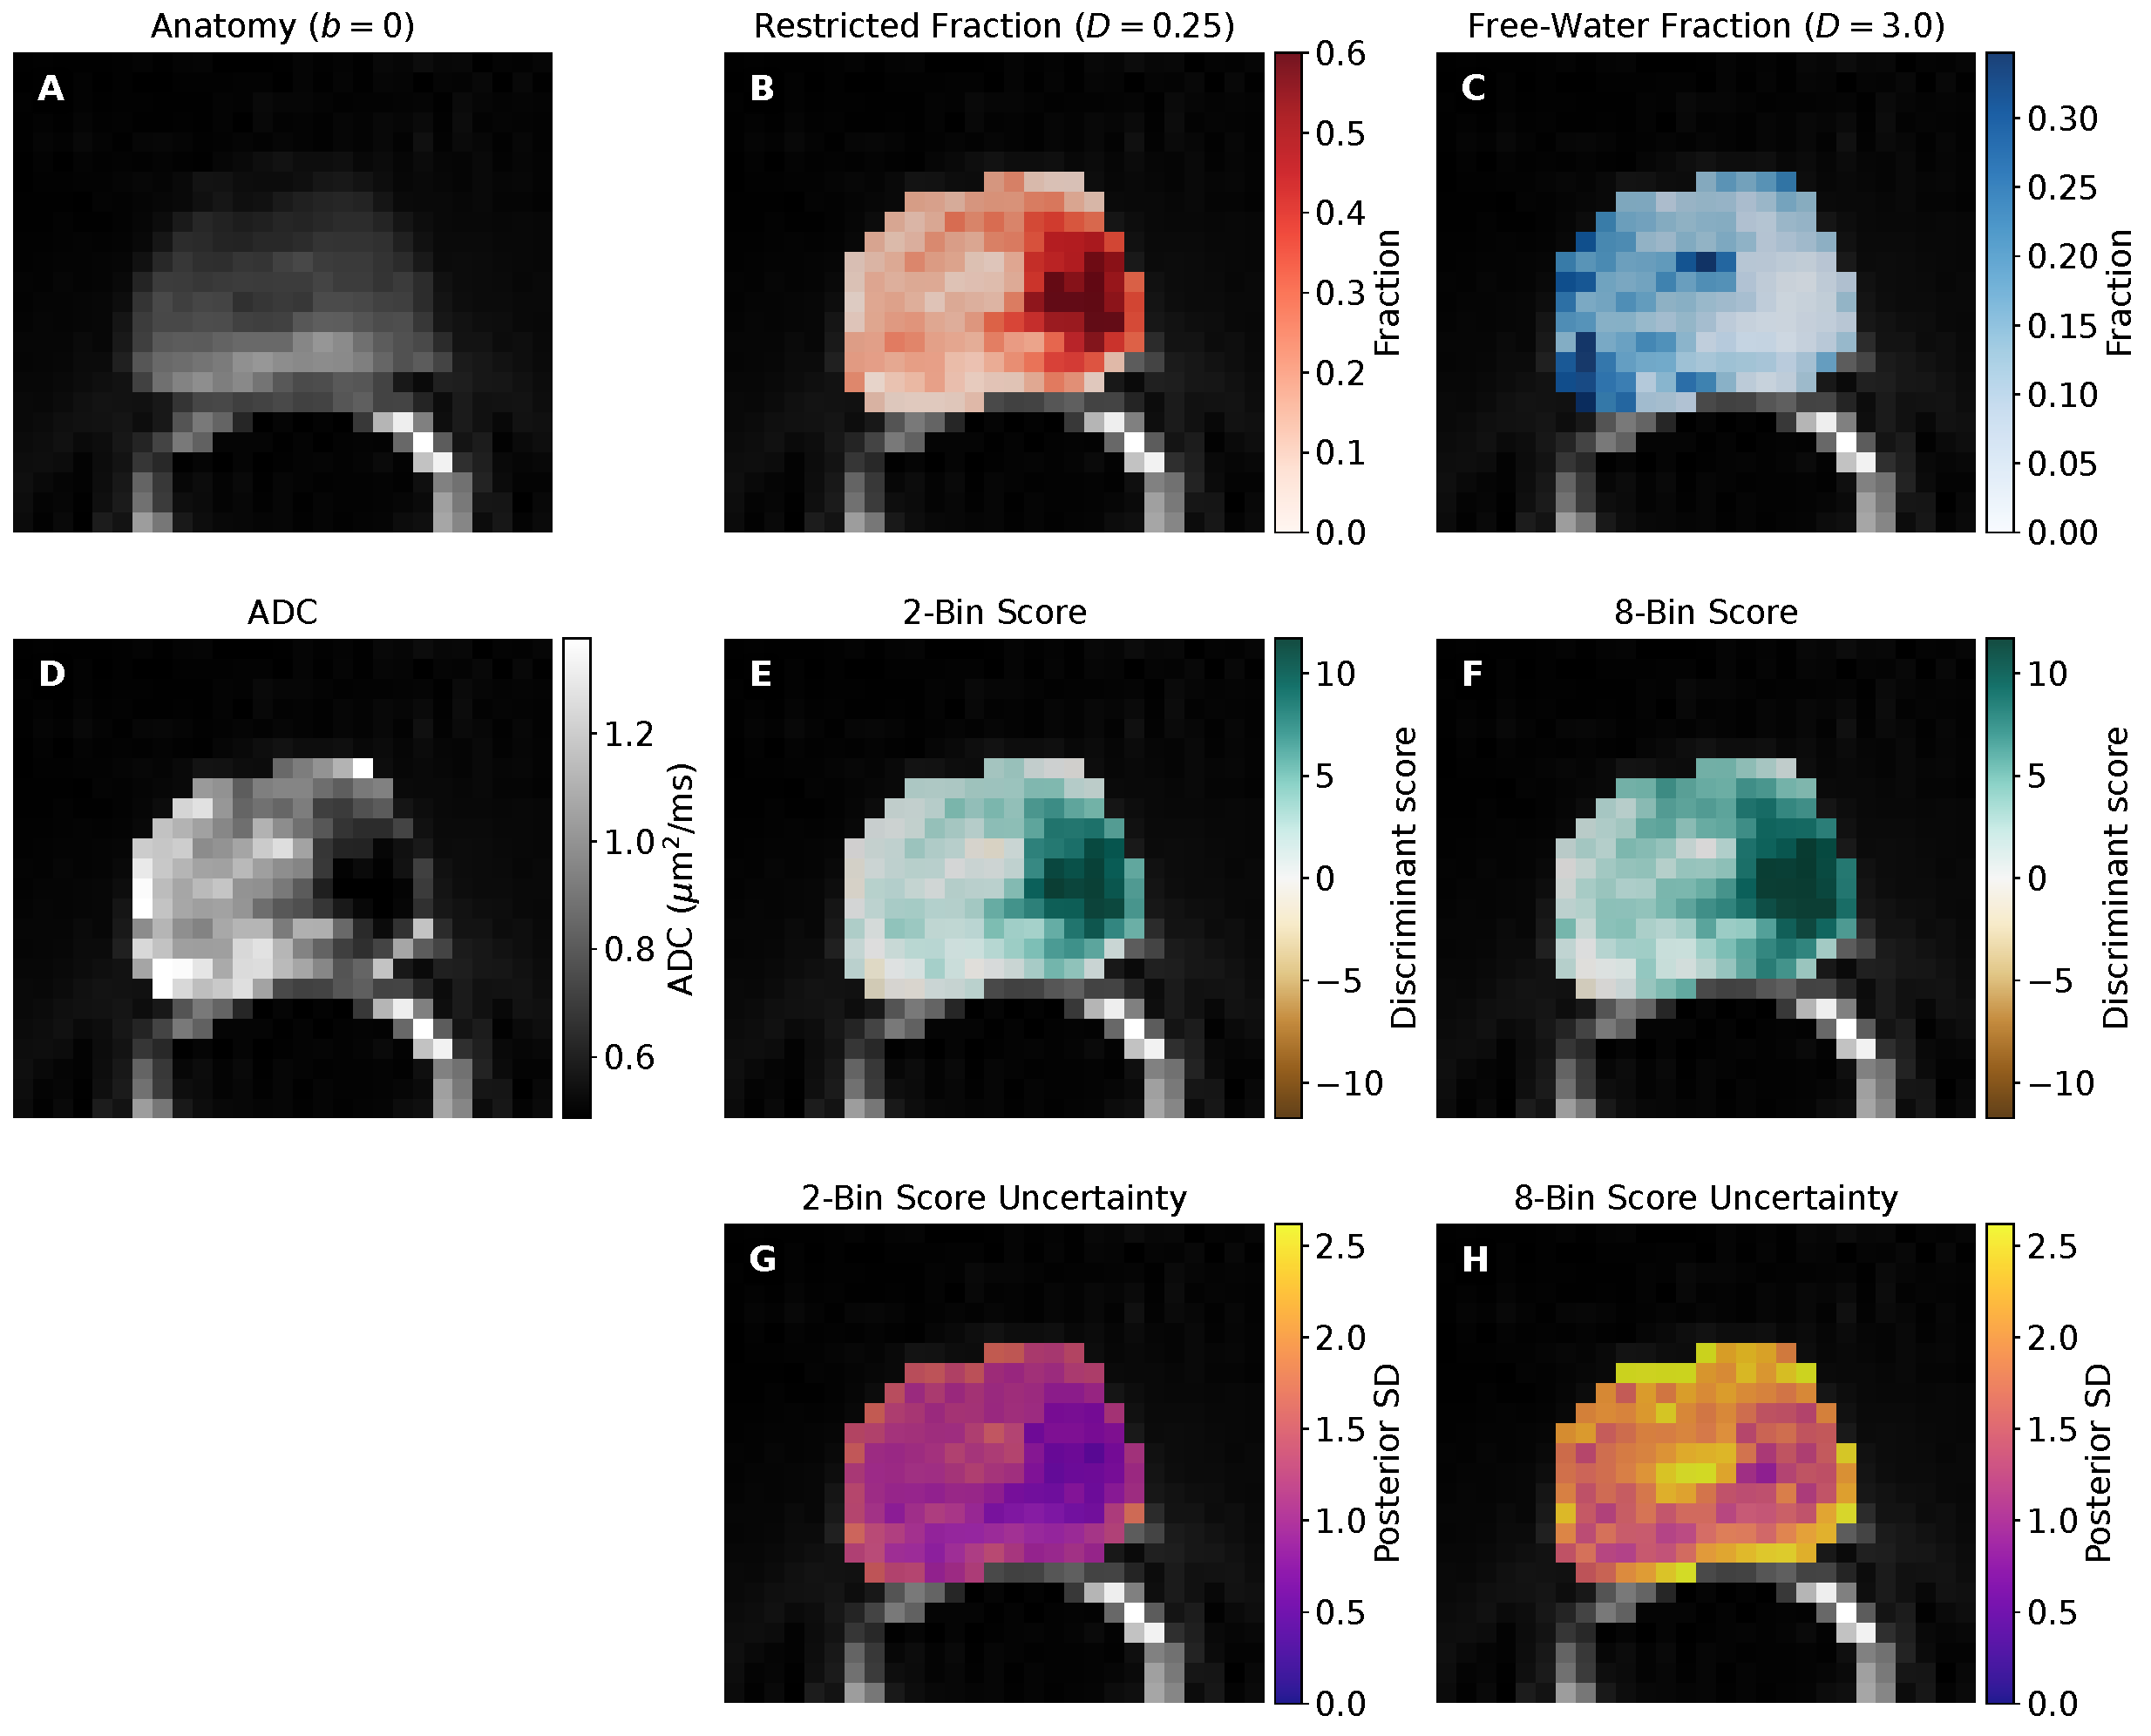
\includegraphics[width=\textwidth]{figures/fig9_v2.pdf}
\caption{%
Pixel-wise spectral decomposition of a single peripheral-zone prostate DWI
slice (anonymized patient), showing that the ROI-level detector extends to the
voxel level while uniquely providing a per-voxel uncertainty map.
(A)~Anatomical reference ($b = 0$).
(B,\,C)~NUTS posterior-mean restricted-diffusion ($D = 0.25\;\umsmm$) and
free-water ($D = 3.0\;\umsmm$) fractions.
(D)~Conventional ADC map (restricted diffusion appears dark).
(E,\,F)~Per-voxel discriminant score for the two-bin
$\{D = 0.25,\,3.0\;\umsmm\}$ and full eight-bin classifiers (peripheral-zone
detectors, same recipe as Fig.~\ref{fig:roc}), centered on the decision
boundary; both reproduce the ADC pattern ($r = -0.93$ and $-0.96$). The
absolute score skews tumor-like because the lower SNR of a single voxel
inflates the restricted fraction, which is why quantitative results are
reported at the ROI level.
(H,\,I)~Posterior standard deviation of the score (500 Monte Carlo draws) for
the two- and eight-bin detectors on a shared scale: the eight-bin map is
$1.8\times$ more uncertain because it weights the unidentifiable intermediate
bins---an uncertainty ADC and point-estimate methods cannot provide.
}
\label{fig:pixelwise}
\end{figure}
